\documentclass{article}
\usepackage[utf8]{inputenc}
\usepackage{graphicx}
\usepackage{amsmath }
\usepackage{amssymb}
\usepackage{subcaption}
\usepackage{float}
\usepackage{mathtools}
\setcounter{section}{0}


\usepackage{cleveref} %referencing figures, equations and tables
\crefformat{figure}{Figure.~#2#1#3}
\crefformat{equation}{Eq.~#2#1#3}
\crefformat{table}{Table.~#2#1#3}
\crefformat{appendix}{Appendix.~#2#1#3}
\crefformat{section}{Section.~#2#1#3}

\title{The Longitudinal Impact of a Rigid Mass Against an Elastic Bar}
\author{Amir Baharvand }
\date{}

\begin{document}

\maketitle

\section{Problem Statement}
\cref{fig:problem} illustrates the longitudinal impact of a rigid mass against an elastic bar. The rigid body has a mass $m_2$ and an initial velocity $v_0$ whereas the elastic bar is fixed at $x=l$ and is free at the origin and has a mass $m_1$, density $\rho$, length $l$ with a cross-sectional area $A$ and Young's modulus $E$. In the following, $c$ is the wave speed.

\begin{figure}[H]
    \centering
    \includegraphics[width = 0.6\textwidth ]{figures/problem_statement.pdf}
    \caption{The problem geometry and coordinate system.}
    \label{fig:problem}
\end{figure}

\section{$0 < ct < 2l$ at $x=0$}
At time interval $0 < ct < 2l$, assuming that $t=0$ is the time when the rigid mass hits the bar, a compressive forward wave $f(ct-x)$ is generated at $x=0$ which takes $t=\dfrac{2l}{c}$ for the generated wave $f_0$ to return to $x=0$. The subscript zero denotes the number given to the generated wave. The displacement, $u$, and strain, $\epsilon$, for this time interval are given here for convenience as it is used later in the subsequent sections.

\begin{align}
    & u_0(x, t) = f_0 = \frac{l v_0}{M c} \left( 1 - e^{-\textstyle\frac{M}{l}ct} \right ) \notag\\ 
    & \epsilon = -\frac{v_0}{c} e^{-\textstyle\frac{M}{l}ct}
    \label{eq:displ_str_t0}
\end{align}

where 

\begin{equation}
    M = \frac{\rho A l}{m_2} = \frac{E A l}{m_2 c^2}
    \label{eq:M}
\end{equation}

\section{$l < ct < 3l$ at $x=l$}
As soon as the compressive backward wave $f_0(ct-x)$ arrives at the fixed boundary ($x=l$), it reflects as a compressive backward wave $g_1(ct+x)$. $g_1$ has a latency of $\dfrac{l}{c}$; therefore, this backward wave is written as $g_!(ct+x-2l)$. Writing and simplifying the relevant equations results in

\begin{equation}
    g_1 = \frac{v_0 l}{c M} \left( e^{-\textstyle\frac{M}{l}(ct+x-2l)} - 1 \right )
    \label{eq:g_1}
\end{equation}

The subscript one represents the generated wave number. 

\section{$2l < ct < 4l$ at $x=0$}
At this time interval, both the forward and backward wave contribute to the displacement and it can be written as

\begin{align}
    u_1(x, t) & = f_1(ct-x-2l) + g_1(ct+x-2l) \notag\\
    & = f_1(\xi_1) + g_1(\xi_2)
    \label{eq:displ_t2l}
\end{align}

in which

\begin{equation*}
    \left\{\begin{matrix}
        \xi_1 = ct - x - 2l\\ 
        \xi_2 = ct + x - 2l
    \end{matrix}\right.
\end{equation*}

In \cref{eq:displ_t2l}, $g_1$ is substituted from \cref{eq:g_1} and $f_1$ is unknown.

\subsection{Determination of $f_1$}
One can write Newton's second law for \cref{fig:problem} for $2l < ct < 4l$ at $x=0$

\begin{align*}
    -m_2 \frac{\partial u^2(x, t)}{\partial t^2} &= -E A \frac{\partial u(x, t)}{\partial x} \\
    m_2 c^2 (f''_1(\xi_1) + g''_1(\xi_2)) &= EA (g'_1(\xi_2) - f'_1(\xi_1))
\end{align*}

where the chain rule is utilized in calculating the derivatives, \emph{i.e.}, $\dfrac{\partial f_1}{\partial \xi_1} \dfrac{\partial \xi_1}{\partial t}$. \\

Because all the above calculations are done at the free end of the bar ($x=0$), $\xi_1$ and $\xi_2$ can be replaced by $\xi = ct-2l$.

\begin{align}
    m_2 c^2 (f''_1(\xi) + g''_1(\xi)) &= EA (g'_1(\xi)- f'_1(\xi)) \notag\\ 
    f''_1(\xi) + g''_1(\xi) &= \frac{M}{l} (g'_1(\xi) - f'_1(\xi))
    \label{eq:ode}
\end{align}

$M$ can be found from \cref{eq:M}. \\

$g_1$ and its derivatives in \cref{eq:ode} can be calculated from \cref{eq:g_1}.

\begin{align*}
    & g'_1(ct + x -2l) = -\frac{v_0}{c} e^{-\textstyle\frac{M}{l}(ct + x -2l)} \\
    & g'_1(\xi)_{\{x=0\}} = -\frac{v_0}{c} e^{-\textstyle\frac{M}{l}\xi} \\
    & g''_1(ct + x -2l) = \frac{M v_0}{l c} e^{-\textstyle\frac{M}{l}(ct + x -2l)} \\
    & g''_1(\xi)_{\{x=0\}} = \frac{M v_0}{l c} e^{-\textstyle\frac{M}{l}\xi} 
\end{align*}

One should note that the above derivatives are taking w.r.t $x$. \\

Replacing $g'_1(\xi)$ and $g''_1(\xi)$ from above set of equations and using the \texttt{dsolve} command from Maple, the solution to \cref{eq:ode} is

\begin{equation}
    f_1(\xi) = \frac{(2 M v_0 \xi - B c l + 2 l v_0)}{M c} e^{-\textstyle\frac{M}{l}\xi} + D
\end{equation}

where $B$ and $D$ are constants and can be determined from initial conditions. In order to find $B$ and $D$, we use the continuity principle of displacements and velocity where both the initial displacement and velocity in \cref{eq:displ_t2l} should have the same value of $u$ and $v$ at $ct = 2l$ in \cref{eq:displ_str_t0}, that is \\

For the displacement:

\begin{align}
    u_1{_{\{x = 0, ct = 2l\}}} &= u_0{_{\{x = 0, ct = 2l\}}}  \notag \\
    f_1{_{\{x = 0, ct = 2l\}}} + g_1{_{\{x = 0, ct = 2l\}}} &= f_0{_{\{x = 0, ct = 2l\}}}
    \label{eq:BD_1}
\end{align}

For the velocity:

\begin{align}
    v_1{_{\{x = 0, ct = 2l\}}} &= v_0{_{\{x = 0, ct = 2l\}}} \notag \\
    \frac{\partial }{\partial t}f_1{_{\{x = 0, ct = 2l\}}} + \frac{\partial }{\partial t}g_1{_{\{x = 0, ct = 2l\}}} &= \frac{\partial }{\partial t}f_0{_{\{x = 0, ct = 2l\}}}
    \label{eq:BD_2}
\end{align}

Solving \cref{eq:BD_1} and \cref{eq:BD_2} simultaneously 

\begin{equation*}
    B = \frac{v_0}{c}(e^{-2M} + 1) \quad , \quad D = 0
\end{equation*}

As a result 

\begin{equation}
    f_1(\xi) = \frac{v_0}{M c} (2 M \xi - l e^{-2M} + l) e^{-\textstyle\frac{M}{l}\xi}
    \label{eq:f_1}
\end{equation}

\section{Displacement and Strain Plots}
The displacement for $2l<ct<4l$ can be found by plugging-in \cref{eq:g_1} and \cref{eq:f_1} into \cref{eq:displ_t2l}.

\begin{equation}
    u_1(x, t) = \frac{v_0}{M c} \left \{ \left[2 M  \left(c t -2 l -x \right)-l \left({ e}^{-2 M}+1\right)+2 l \right] { e}^{-\textstyle\frac{M}{l}(c t -2 l -x)} + l \left({ e}^{-\textstyle\frac{M}{l}(c t -2 l + x)}-1\right) \right \}
    \label{eq:displ_t2l_complete}
\end{equation}

\cref{fig:displ} shows the piecewise combination of \cref{eq:displ_str_t0} and \cref{eq:displ_t2l_complete} for $0<ct<4l$ for $c = 1$, $ l = 1$,  $M = 1$ at the free side of the elastic bar ($x = 0$). As expected, the displacement plot is continuous. \\

The strain can be calculated by taking the derivative of displacements from \cref{eq:displ_str_t0} and \cref{eq:displ_t2l_complete} w.r.t $x$.

\begin{equation}\resizebox{1\hsize}{!}{$
    \begin{cases}
        \epsilon_0 = \dfrac{v_0}{c} e^{-\textstyle\frac{M}{l}ct} & , 0<ct<2l \\
        \\
        \epsilon_1 = \dfrac{v_0}{c} \left \{ \left ( \dfrac{2M(ct-2l-x) - l(e^{-2M} + 1) + 2l}{l} -2 \right ) e^{-\textstyle\frac{M}{l}(ct-2l-x)} - e^{-\textstyle\frac{M}{l}(ct-2l+x)} \right \} & , 2l<ct<4l
    \end{cases}$}
    \label{eq:strains}
\end{equation}

\cref{eq:strains} is plotted in \cref{fig:strain}. As it is seen, the discontinuity in the strain plot occurs at $t=2l$ where the strain jumps to higher but negative value. It is also evident that for $0<ct<2l$, the strain does not become zero as it appears in form of an exponential function (see \cref{eq:strains}$_1$), while the strain and subsequently the stress (due to linear elastic assumption between stress and strain) vanishes at around $3l$. To find  the corresponding time, we may solve \cref{eq:strains}$_2$ for $t$.

\begin{equation*}
    t = \dfrac{1}{2} \dfrac{4 M l +2 M x +l e^{-2 M}+l +l e^{-\textstyle\frac{2 M}{l}x}}{M c}
\end{equation*}

If we remove $x$ from above equation

\begin{equation}
    t = \dfrac{1}{2} \dfrac{4 M l +l \,{ e}^{-2 M}+2 l}{M c}
\end{equation}

and for $c = 1$, $ l = 1$,  $M = 1$, the time at which stress vanishes is 3.068s.


\begin{figure}[H]
    \centering
    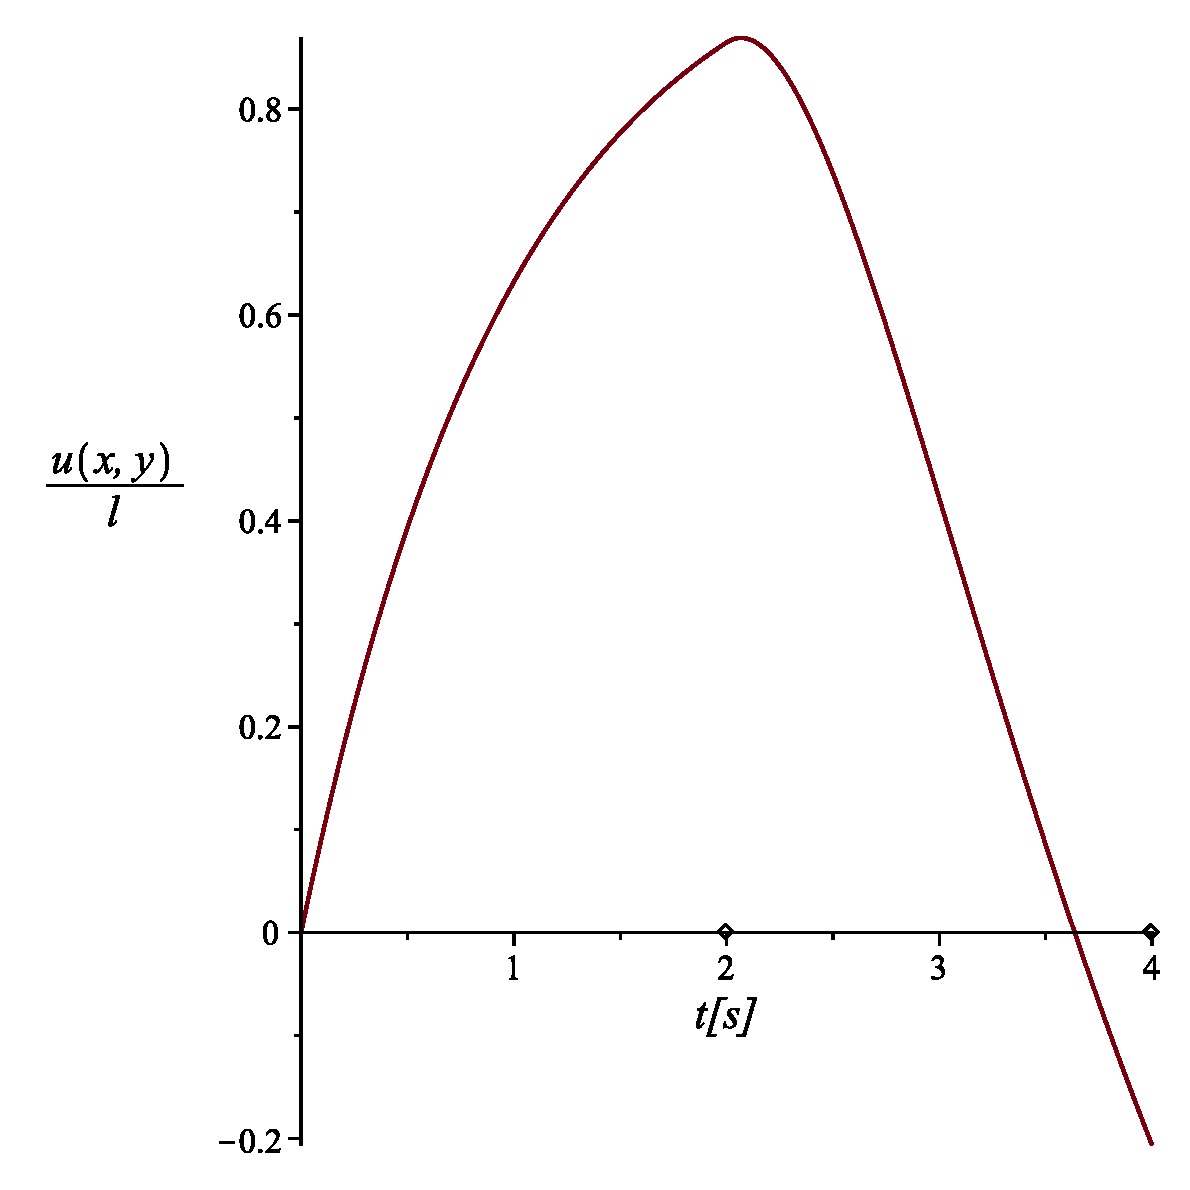
\includegraphics[width = 0.6\textwidth ]{figures/displ.eps}
    \caption{Normalized displacement against time for $c = 1$, $ l = 1$,  $M = 1$ at the free side of the elastic bar ($x = 0$).}
    \label{fig:displ}
\end{figure}


\begin{figure}[H]
    \centering
    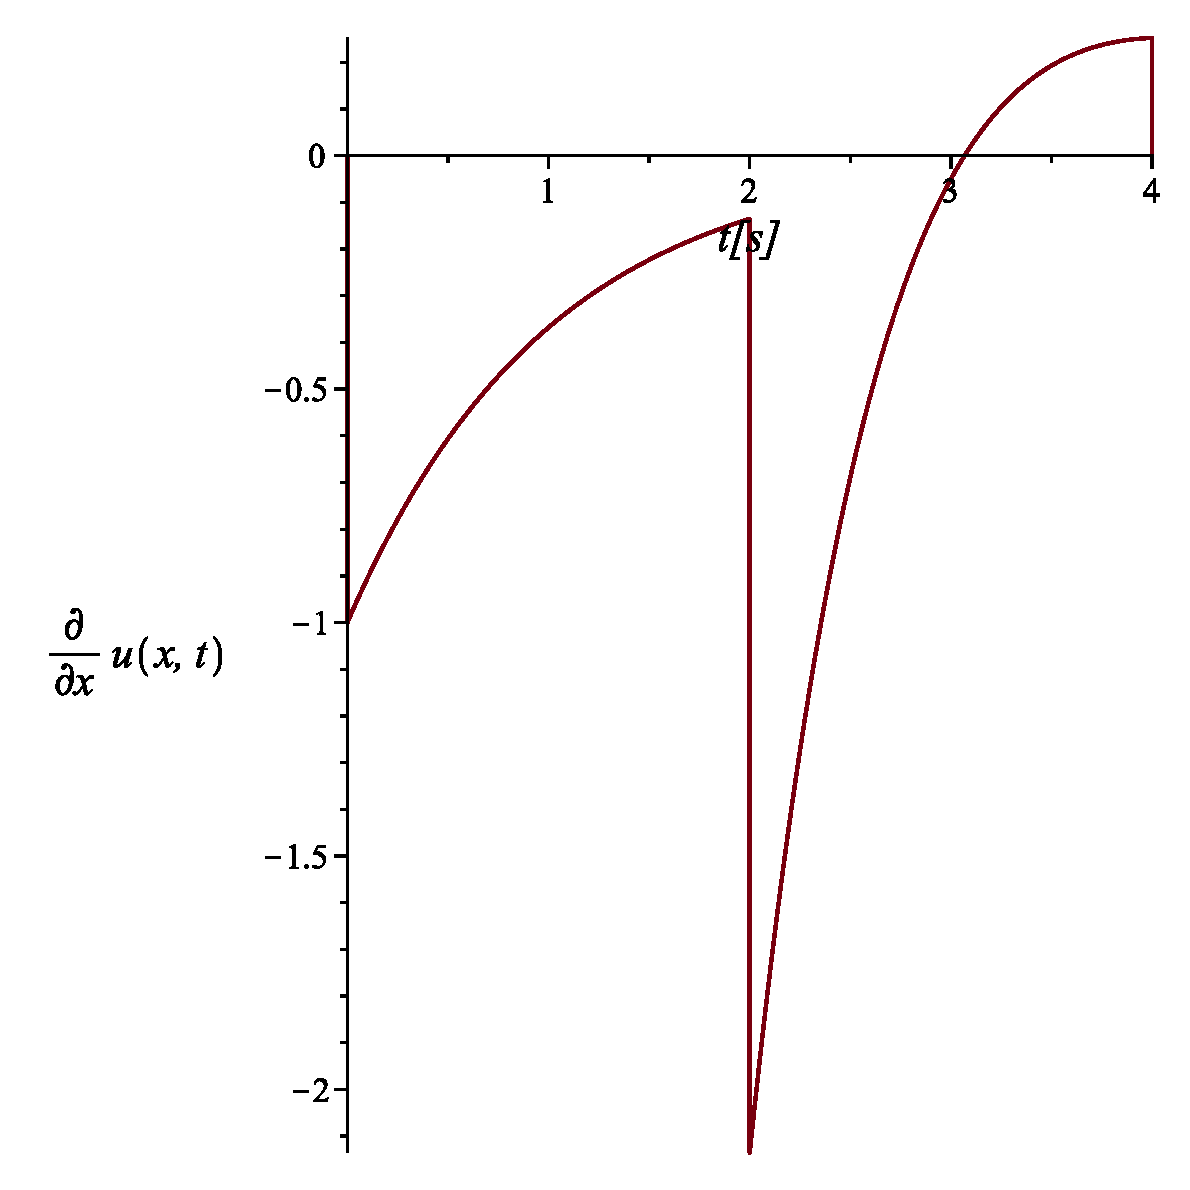
\includegraphics[width = 0.6\textwidth ]{figures/strain.eps}
    \caption{Strain against time for $c = 1$, $ l = 1$,  $M = 1$ at the free side of the elastic bar ($x = 0$).}
    \label{fig:strain}
\end{figure}


% \newpage
% \bibliography{ref}
% \bibliographystyle{ieeetr}

\end{document}